\section{Evaluación del comportamiento}

Se ha probado a construir tanto el mapa del entorno de la clase como el del pasillo, con éxito en ambos casos. Sin embargo, es notable que los movimientos muy veloces y los giros rápidos provocan errores considerables que quedan reflejados en el dibujo del mapa.

En la Figura \ref{fig:clase} se observa una de las pruebas realizadas para el construir el mapa de la clase.

\begin{figure}[h]
    \centering
    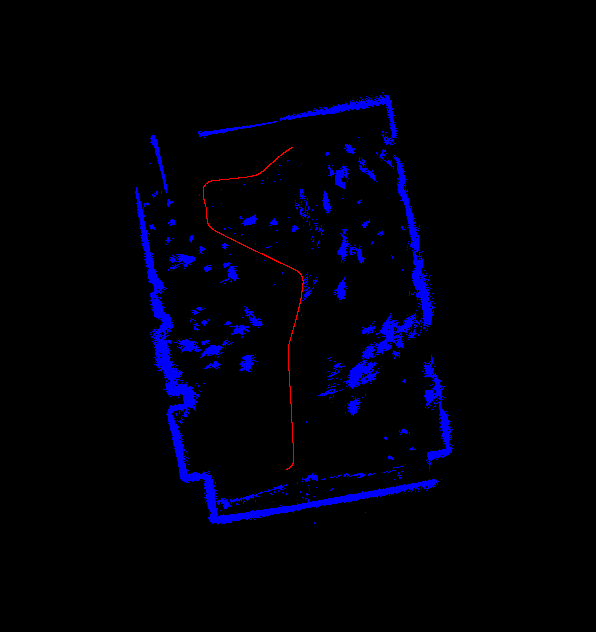
\includegraphics[scale=0.35]{images/mapa_clase.png}
    \caption{Mapa de la clase. La esquina superior izquierda correspondería a la entrada de la misma.}
    \label{fig:clase}
\end{figure}